\documentclass{beamer}

% hide navigation symbols
\setbeamertemplate{navigation symbols}{}

\usepackage[export]{adjustbox}

\title{Math 802: Intro to Course Tools}   
\author{Nathan Albin} 
\date{\today} 


\begin{document}

\frame{\titlepage} 

\begin{frame}{Before git}
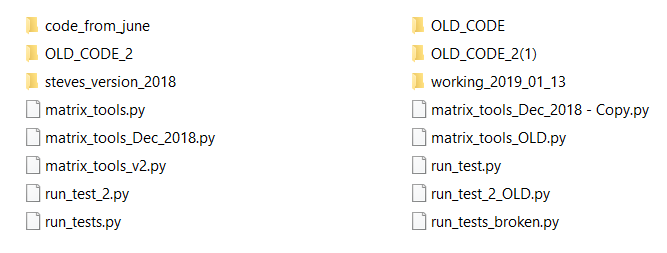
\includegraphics[width=\textwidth]{images/folder_pre_git.png}
\end{frame}

\begin{frame}{After git}

\includegraphics[width=0.25\textwidth,valign=t]{images/folder_post_git.png}%
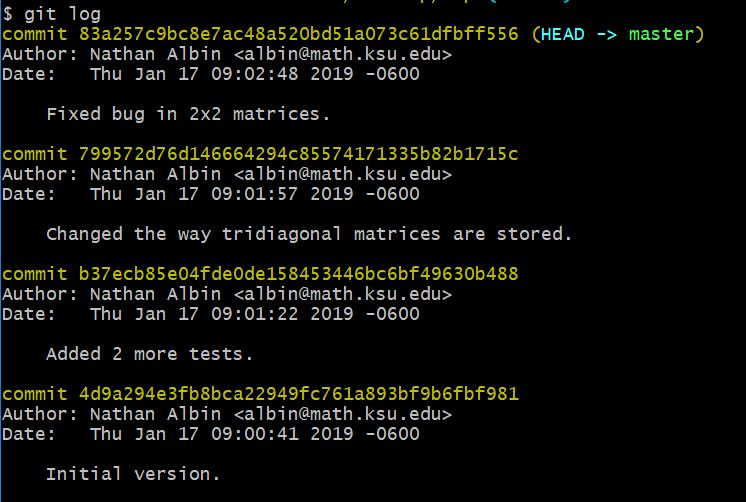
\includegraphics[width=0.7\textwidth,valign=t]{images/git_log.png}
\end{frame}

\begin{frame}{Managing repositories on GitHub}
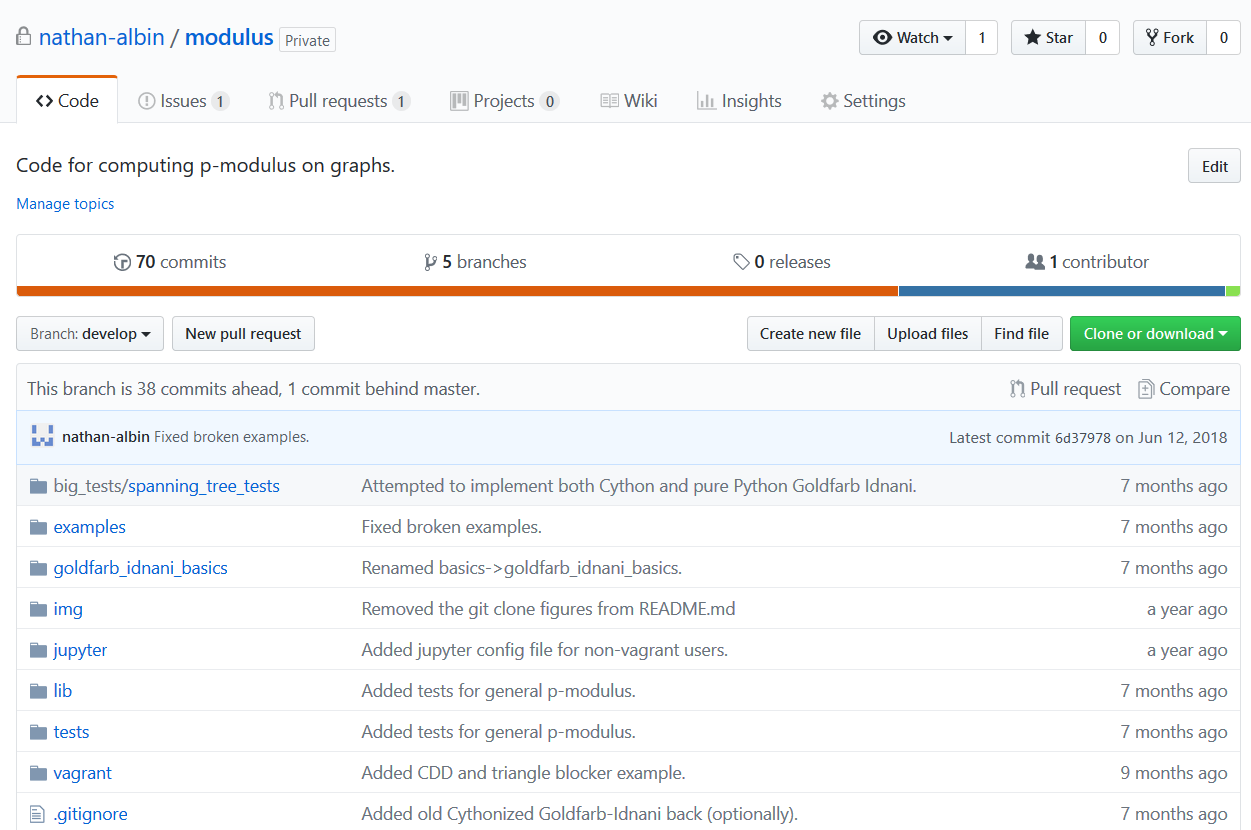
\includegraphics[width=\textwidth]{images/github.png}
\end{frame}

\begin{frame}{Static code analysis with pylint}
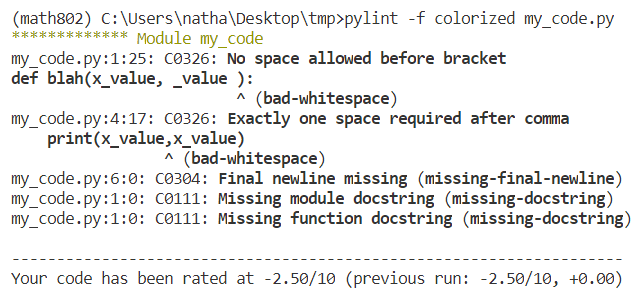
\includegraphics[width=0.85\textwidth]{images/pylint.png}
\end{frame}

\begin{frame}{Testing with pytest}
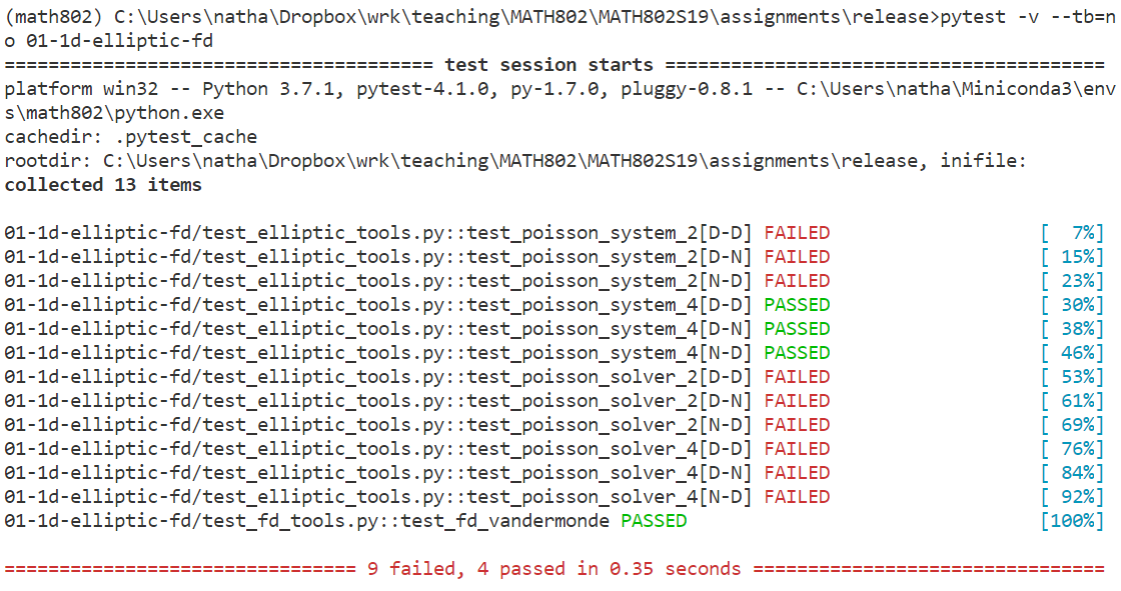
\includegraphics[width=0.95\textwidth]{images/pytest.png}
\end{frame}

\end{document}
